\documentclass[14pt,a4paper]{report}  %紙張設定
\usepackage{xeCJK}%中文字體模組
%\setCJKmainfont{標楷體} %設定中文字體
\setCJKmainfont{MoeStandardKai.ttf}
%\newfontfamily\sectionef{Times New Roman}%設定英文字體
\newfontfamily\sectionef{Nimbus Roman}
\usepackage{enumerate}
\usepackage{amsmath,amssymb}%數學公式、符號
\usepackage{amsfonts} %數學簍空的英文字
\usepackage{graphicx, subfigure}%圖形
\usepackage{fontawesome5} %引用icon
\usepackage{type1cm} %調整字體絕對大小
\usepackage{textpos} %設定文字絕對位置
\usepackage[top=2.5truecm,bottom=2.5truecm,
left=3truecm,right=2.5truecm]{geometry}
\usepackage{titlesec} %目錄標題設定模組
\usepackage{titletoc} %目錄內容設定模組
\usepackage{textcomp} %表格設定模組
\usepackage{multirow} %合併行
%\usepackage{multicol} %合併欄
\usepackage{CJK} %中文模組
\usepackage{CJKnumb} %中文數字模組
\usepackage{wallpaper} %浮水印
\usepackage{listings} %引用程式碼
\usepackage{hyperref} %引用url連結
\usepackage{setspace}
\usepackage{lscape}%設定橫式
\lstset{language=Python, %設定語言
		basicstyle=\fontsize{10pt}{2pt}\selectfont, %設定程式內文字體大小
		frame=lines,	%設定程式框架為線
}
%\usepackage{subcaption}%副圖標
\graphicspath{{./../images/}} %圖片預設讀取路徑
\usepackage{indentfirst} %設定開頭縮排模組
\renewcommand{\figurename}{\Large 圖.} %更改圖片標題名稱
\renewcommand{\tablename}{\Large 表.}
\renewcommand{\lstlistingname}{\Large 程式.} %設定程式標示名稱
\hoffset=-5mm %調整左右邊界
\voffset=-8mm %調整上下邊界
\setlength{\parindent}{3em}%設定首行行距縮排
\usepackage{appendix} %附錄
\usepackage{diagbox}%引用表格
\usepackage{multirow}%表格置中
%\usepackage{number line}
%=------------------更改標題內容----------------------=%
\titleformat{\chapter}[hang]{\center\sectionef\fontsize{20pt}{1pt}\bfseries}{\LARGE 第\CJKnumber{\thechapter}章}{1em}{}[]
\titleformat{\section}[hang]{\sectionef\fontsize{18pt}{2.5pt}\bfseries}{{\thesection}}{0.5em}{}[]
\titleformat{\subsection}[hang]{\sectionef\fontsize{18pt}{2.5pt}\bfseries}{{\thesubsection}}{1em}{}[]
%=------------------更改目錄內容-----------------------=%
\titlecontents{chapter}[11mm]{}{\sectionef\fontsize{18pt}{2.5pt}\bfseries\makebox[3.5em][l]
{第\CJKnumber{\thecontentslabel}章}}{}{\titlerule*[0.7pc]{.}\contentspage}
\titlecontents{section}[18mm]{}{\sectionef\LARGE\makebox[1.5em][l]
{\thecontentslabel}}{}{\titlerule*[0.7pc]{.}\contentspage}
\titlecontents{subsection}[4em]{}{\sectionef\Large\makebox[2.5em][l]{{\thecontentslabel}}}{}{\titlerule*[0.7pc]{.}\contentspage}
%=----------------------章節間距----------------------=%
\titlespacing*{\chapter} {0pt}{0pt}{18pt}
\titlespacing*{\section} {0pt}{12pt}{6pt}
\titlespacing*{\subsection} {0pt}{6pt}{6pt}
%=----------------------標題-------------------------=%             
\begin{document} %文件
\sectionef %設定英文字體啟用
\vspace{12em}
\begin{titlepage}%開頭
\begin{center}   %標題  
\makebox[1.5\width][s] %[s] 代表 Stretch the interword space in text across the entire width
{\fontsize{24pt}{2.5pt}國立虎尾科技大學}\\[18pt]
\makebox[1.5\width][s]
{\fontsize{24pt}{2.5pt}機械設計工程系}\\[18pt]
\sectionef\fontsize{24pt}{1em}\selectfont\textbf
{
\vspace{0.5em}
cd2023 2a3-pj3ag2分組報告}\\[18pt]
%設定文字盒子 [方框寬度的1.5倍寬][對其方式為文字平均分分布於方框中]\\距離下方18pt
\vspace{1em} %下移
\fontsize{30pt}{1pt}\selectfont\textbf{網際足球泡泡機器人場景設計}\\
\vspace{1em}
\sectionef\fontsize{30pt}{1em}\selectfont\textbf
{
\vspace{0.5em}
Web-based bubbleRob Football Scene Design}
 \vspace{2em}
%=---------------------參與人員-----------------------=%             
\end{center}
\begin{flushleft}
\begin{LARGE}

\hspace{32mm}\makebox[5cm][s]
{指導教授:\quad 嚴\quad 家\quad 銘\quad 老\quad 師}\\[6pt]
\hspace{32mm}\makebox[5cm][s]
{班\qquad 級:\quad 四\quad 設\quad 二\quad 甲}\\[6pt]
\hspace{32mm}\makebox[5cm][s]
{學\qquad 生:\quad 江\quad 芷\quad 柔\quad(41023103)}\\[6pt]
\hspace{32mm}\makebox[5cm][s]
{\hspace{36.5mm}李\quad 凱\quad 新\quad(41023106)}\\[6pt]
\hspace{32mm}\makebox[5cm][s]
{\hspace{36.5mm}王\quad 翔\quad 楷\quad(41023113)}\\[6pt]
\hspace{32mm}\makebox[5cm][s]
{\hspace{36.5mm}吳\quad 勁\quad 毅\quad(41023116)}\\[6pt]
\hspace{32mm}\makebox[5cm][s]
{\hspace{36.5mm}李\quad 學\quad 淵\quad(41023125)}\\[6pt]
\hspace{32mm}\makebox[5cm][s]
{\hspace{36.5mm}林\quad 秉\quad 賢\quad(41023132)}\\[6pt]
\hspace{32mm}\makebox[5cm][s]
{\hspace{36.5mm}張\quad 育\quad 銓\quad(41023151)}\\[6pt]
\hspace{32mm}\makebox[5cm][s]
{\hspace{36.5mm}張\quad 昱\quad 棠\quad(41023153)}\\[6pt]
%設定文字盒子[寬度為5cm][對其方式為文字平均分分布於方框中]空白距離{36.5mm}\空白1em
\end{LARGE}
\end{flushleft}
\vspace{3em}
\fontsize{18pt}{2pt}\selectfont\centerline{\makebox[\width][s]
{中華民國\hspace{3em} 
112 \quad 年\quad 5\quad 月}}
\end{titlepage}
\newpage


%=------------------------摘要-----------------------=%
\renewcommand{\baselinestretch}{1.5} %設定行距
\pagenumbering{roman} %設定頁數為羅馬數字
\clearpage  %設定頁數開始編譯
\sectionef
\addcontentsline{toc}{chapter}{摘~~~要} %將摘要加入目錄
\begin{center}
\LARGE\textbf{摘~~要}\\
\end{center}
\begin{flushleft}
\fontsize{14pt}{20pt}\sectionef\hspace{12pt}\quad 由於矩陣計算、自動求導技術、開源開發環境、多核GPU運算硬體等這四大發展趨勢,促使AI領域快速發展,藉由這樣的契機,將實體機電系統透過虛擬化訓練提高訓練效率,再將訓練完的模型應用到實體上。\\[12pt]

\fontsize{14pt}{20pt}\sectionef\hspace{12pt}\quad 此專題是運用實體冰球對打機,將其導入CoppeliaSim模擬環境並給予對應設置,將其機電系統簡化並運用Open AI Gym進行訓練,找到適合此系統的演算法後,再到CoppeliaSim模擬環境中進行測試演算法在實際運用上的可行性。並嘗試透過架設伺服器將CoppeliaSim影像串流到網頁供使用者觀看或操控。\\[12pt]

\end{flushleft}
\begin{center}
\fontsize{14pt}{20pt}\selectfont 關鍵字: 類神經網路、強化學習、\sectionef CoppeliaSim、OpenAI Gym
\end{center}
\newpage
%=--------------------Abstract----------------------=%
\renewcommand{\baselinestretch}{1.5} %設定行距
\addcontentsline{toc}{chapter}{Abstract} %將摘要加入目錄
\begin{center}
\LARGE\textbf\sectionef{Abstract}\\
\begin{flushleft}
\fontsize{14pt}{16pt}\sectionef\hspace{12pt}\quad Due to the four major development trends of multidimensional arrays  computing, automatic differentiation, open source development environment, and multi-core GPUs computing hardware. The rapid development of the AI field has been promoted. In view of this development, the physical mechatronic systems can gain machine learning efficiency through their simulated virtual system training process. And afterwards to apply the trained model into real mechatronic systems.\\[12pt]

\fontsize{14pt}{16pt}\sectionef\hspace{12pt}\quad This project is to use the physical air hockey to play machine, introduce it into the CoppeliaSim simulation environment and give the corresponding settings, simplify its electromechanical system and use Open AI Gym for training, find an algorithm suitable for this system, and then perform it in the CoppeliaSim simulation environment Feasibility of testing algorithm in practical application. And try to stream CoppeliaSim images to web pages for users to watch or manipulate by setting up a server.\\
\end{flushleft}
\begin{center}
\fontsize{14pt}{16pt}\selectfont\sectionef Keyword:  nerual network、reinforcement learning、 CoppeliaSim、OpenAI Gym
\end{center}
\newpage
%=------------------------誌謝----------------------=%
%=------------------------目錄----------------------=%
\renewcommand{\contentsname}{\centerline{\fontsize{18pt}{\baselineskip}\selectfont\textbf{目\quad 錄}}}
\tableofcontents  %目錄產生
\newpage
%=------------------圖表目錄產生----------------------=%
\renewcommand{\listfigurename}{\centerline{\fontsize{18pt}{\baselineskip}\selectfont\textbf{圖\quad 目\quad 錄 }}}
\newcommand{\loflabel}{圖} %定義\loflabel 文字為圖
\renewcommand{\numberline}[1]{\loflabel~#1\hspace*{0.5em}}
\listoffigures
%\newcommand{\captioname}{圖}
\end{center}
%=-------------------------內容----------------------=%
\chapter{前言}
\renewcommand{\baselinestretch}{10.0} %設定行距
\pagenumbering{arabic} %設定頁號阿拉伯數字
\setcounter{page}{1}  %設定頁數
\fontsize{14pt}{2.5pt}\sectionef
\section{規則}
遊戲規則如下:
\begin{enumerate}
\item 球打入敵方即得一分。
\item 時間內進球數多的一方獲勝。
\end{enumerate}
\renewcommand{\baselinestretch}{0.5} %設定行距
\chapter{場景建立}
\section{前言}
因為這次老師重新規劃了球場及球員的大小、重量......等等,我們重新規劃了整個球場及新建了球員模型,沒有沿用過去的設計。\\
\section{建立球員}
我們使用Onshape重新繪製了球員模型,這次規劃想改變過去bubbleRob看起來較呆版,圓潤的設計,因此設計了一台跑車作為我們的球員。File-Import-Mesh,選擇要匯入的檔案匯入球場,如(圖.\ref{球員建立}) 。接著加入joint\\
加入joint:滑鼠右鍵-Add-Joint-Revolute\\
\
\begin{figure}[hbt!]
\begin{center}
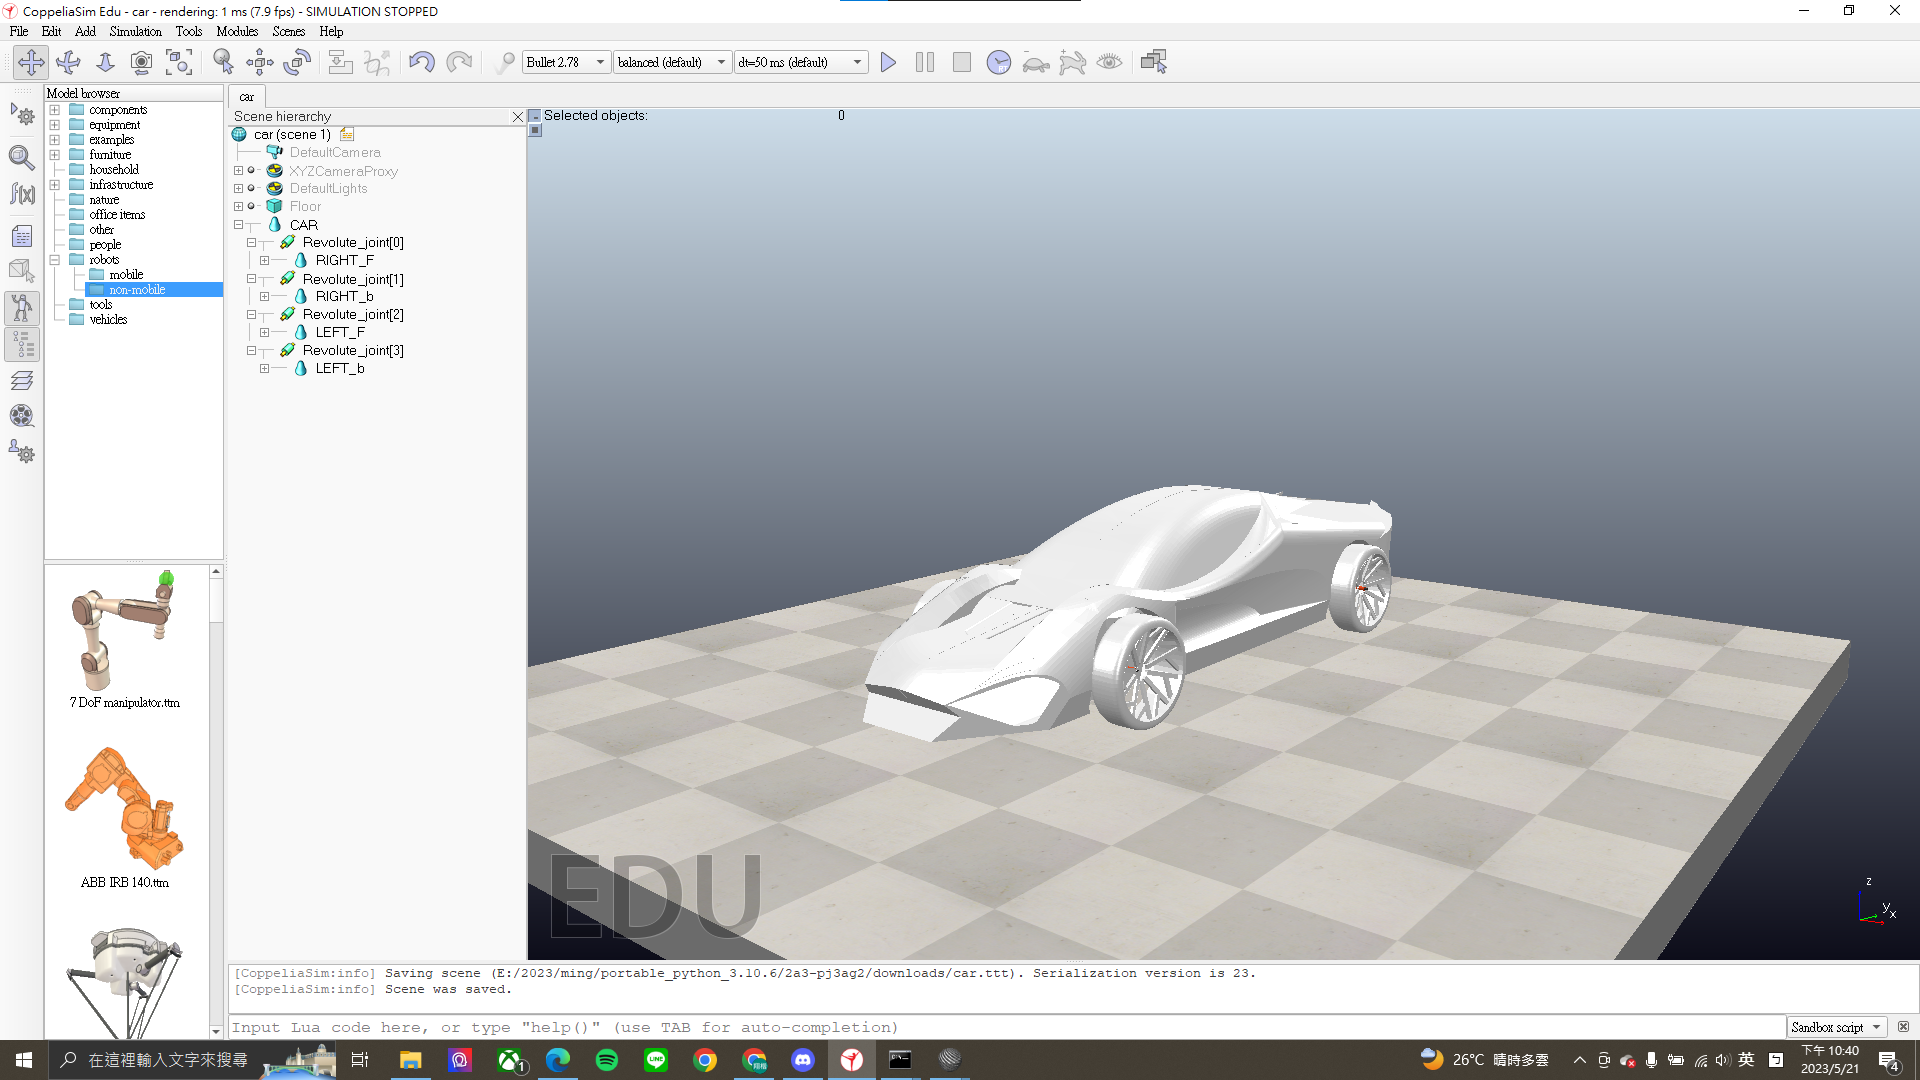
\includegraphics[width=12cm]{球員}
\caption{\Large 球員建立}\label{球員建立}
\end{center}
\end{figure}
\\
\
後發現比例錯誤,因此直接在CoppeliaSim內進行縮小,但因本來設計的跑車高度太低太扁平,可能會有無法推到球的狀況發生,因此不是使用等比縮小,而是直接將各部分拉至規定尺寸。如(圖.\ref{球員建立2})\\
\
比例放大縮小步驟:點選物件左邊圖示-View modify geornrtry-若勾選Keep proportions為進行等比放大,若取消勾選擇可以個別調整大小。\
\begin{figure}[hbt!]
\begin{center}
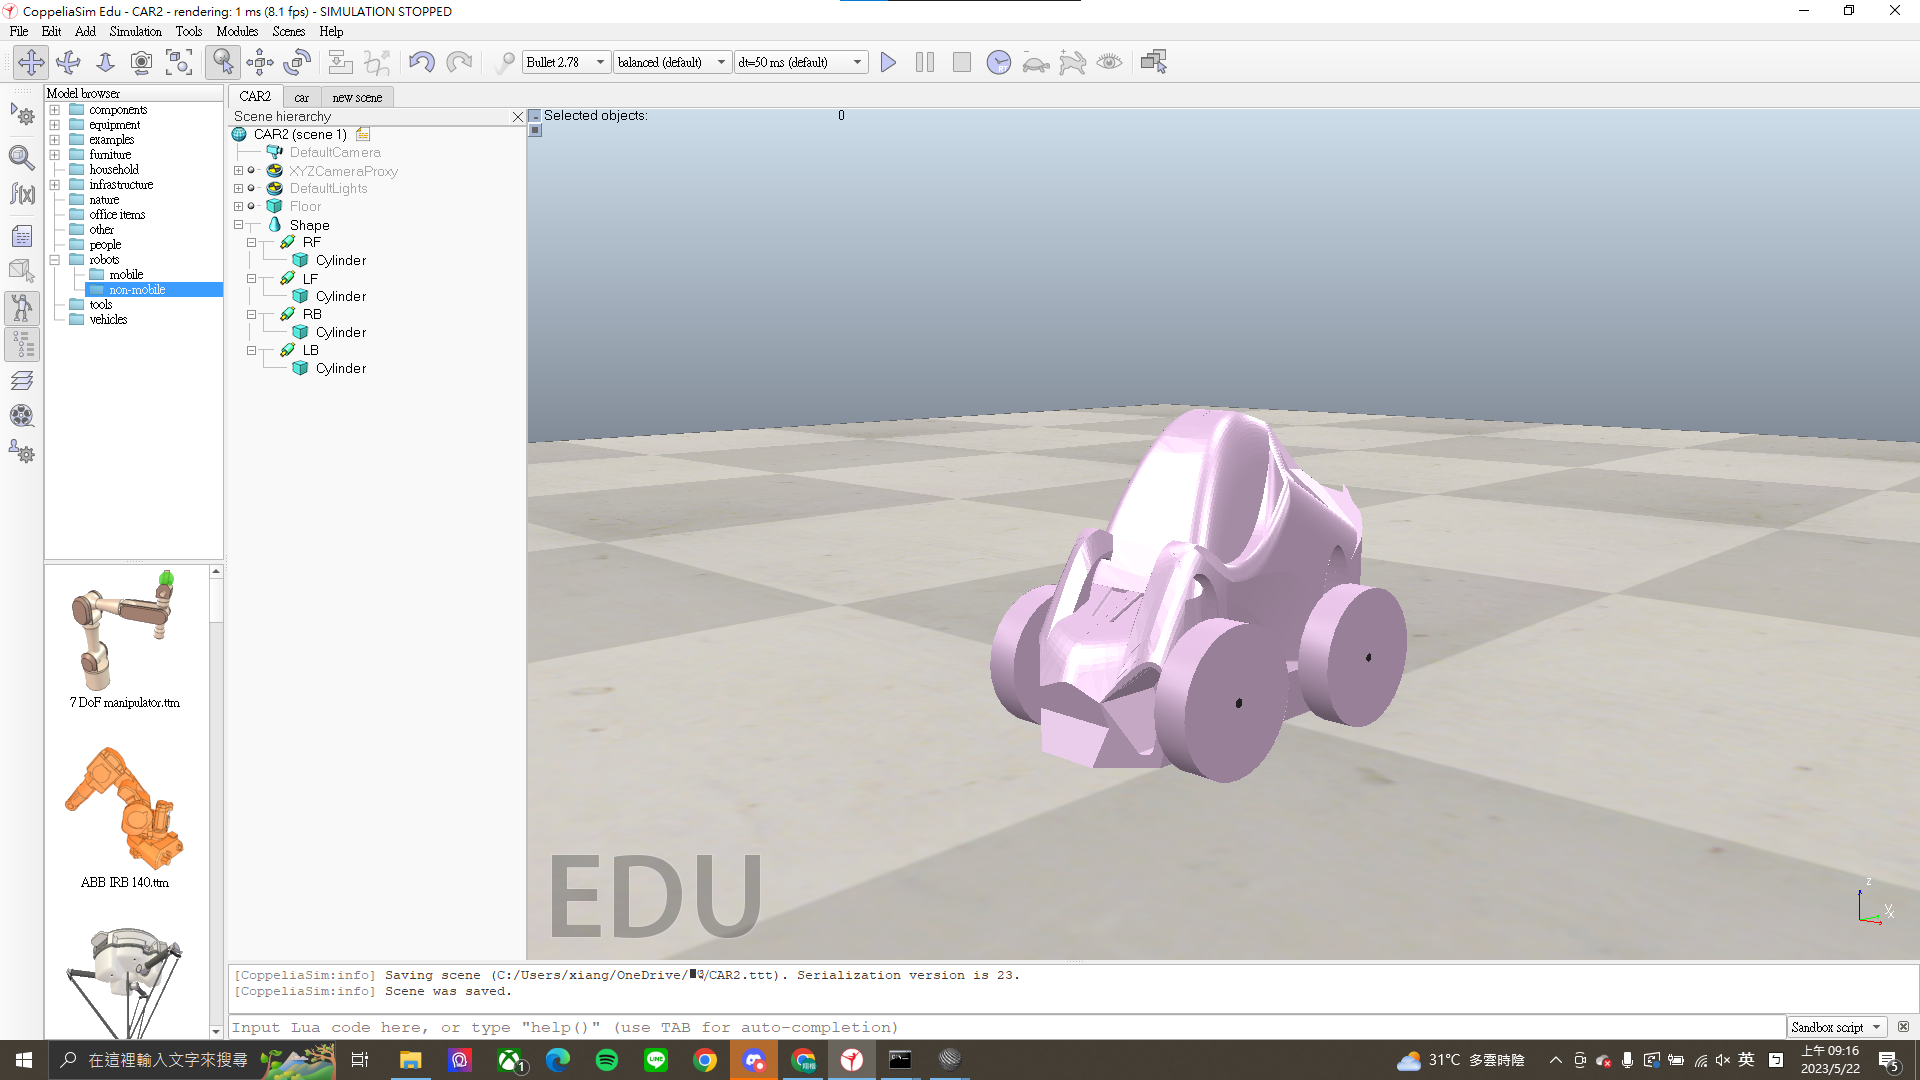
\includegraphics[width=12cm]{球員2}
\caption{\Large 球員建立2}\label{球員建立2}
\end{center}
\end{figure}\
\newpage
\chapter{程式講解}
\section{設定句柄變數}
\begin{figure}[hbt!]
\begin{center}
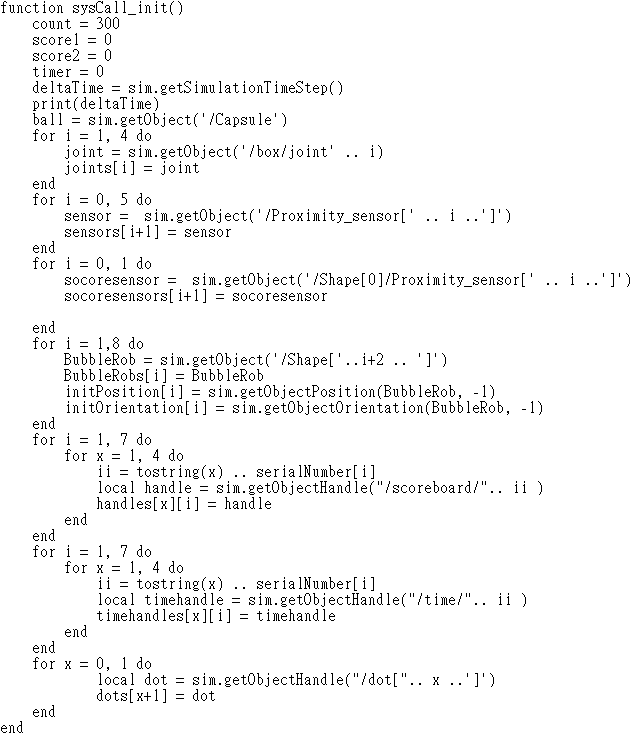
\includegraphics[width=12cm]{1}
\caption{\Large 設定句柄變數}\label{設定句柄變數}
\end{center}
\end{figure} 
這段程式碼,如(圖.\ref{設定句柄變數}),功能性及註解,如(圖.\ref{設定句柄變數註解})\
\begin{figure}[hhtbp!]
\begin{center}
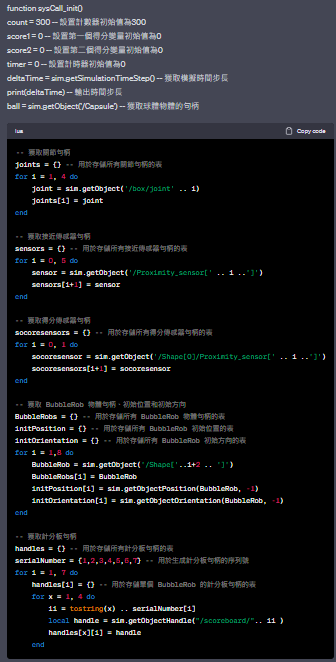
\includegraphics[width=12cm]{1解說}
\caption{\Large 設定句柄變數註解}\label{設定句柄變數註解}
\end{center}
\end{figure}
\
\newpage
\
\section{回復記分板顏色}
\begin{figure}[htbp!]
\begin{center}
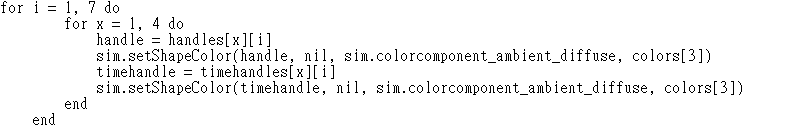
\includegraphics[width=12cm]{2}
\caption{\Large 回復記分板顏色}\label{回復記分板顏色}
\end{center}
\end{figure} 
\
這段程式碼,如(圖.\ref{回復記分板顏色}),四、六行註解為設置計分板形狀的顏色為 color3。
\section{產生隨機座標}
\begin{figure}[htbp!]
\begin{center}
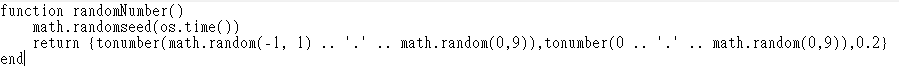
\includegraphics[width=12cm]{3}
\caption{\Large 產生隨機座標}\label{產生隨機座標}
\end{center}
\end{figure} 
\
這段程式碼,如(圖.\ref{產生隨機座標}),第二行註解為使用當前時間作為隨機亂數。
\section{設定記分板顏色}
\begin{figure}[htbp!]
\begin{center}
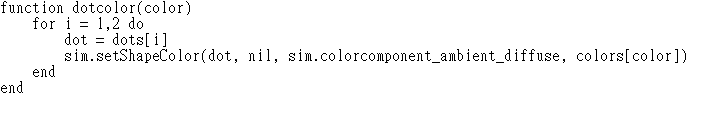
\includegraphics[width=12cm]{4}
\caption{\Large 設定記分板顏色}\label{設定記分板顏色}
\end{center}
\end{figure} 
\
這個函式,如(圖.\ref{設定記分板顏色})用於設置兩個點的顏色。它接受一個參數 color,用於指定要設置的顏色。在函式內部,使用 sim.setShapeColor 函式將顏色應用到每個點的形狀上,使用 colors[color] 來獲取指定的顏色。
\section{分解剩餘時間數字}
\begin{figure}[htbp!]
\begin{center}
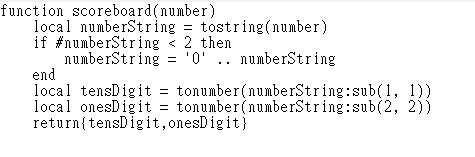
\includegraphics[width=12cm]{5}
\caption{\Large 分解剩餘時間數字}\label{分解剩餘時間數字}
\end{center}
\end{figure} 
\
這個函式,如(圖.\ref{分解剩餘時間數字})用於將數字轉換為計分板的十位數和個位數。它接受一個參數 number,代表要轉換的數字。首先,將數字轉換為字符串 numberString。如果 numberString 的長度小於 2,則在前面添加一個 '0',確保有兩位數字。然後,使用 tonumber 和 string.sub 函式提取十位數和個位數,分別存儲在 tensDigit 和 onesDigit 中。最後,返回一個包含十位數和個位數的數組。
\section{感測得分並修改記分板}
\begin{figure}[htbp!]
\begin{center}
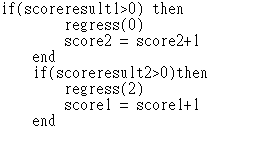
\includegraphics[width=12cm]{6}
\caption{\Large 感測得分並修改記分板}\label{感測得分並修改記分板}
\end{center}
\end{figure} 
\
這個函式,如(圖.\ref{感測得分並修改記分板})包含兩個條件語句。第一個條件語句檢查 scoreresult1 是否大於 0,如果是,則執行 regress(0) 函式並將 score2 加一。第二個條件語句檢查 scoreresult2 是否大於 0,如果是,則執行 regress2)函式並將 score1 加一。
\newpage
\section{將即時分數顯示在計分板}
\begin{figure}[htbp!]
\begin{center}
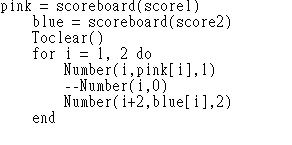
\includegraphics[width=12cm]{7}
\caption{\Large 將即時分數顯示在計分板}\label{將即時分數顯示在計分板}
\end{center}
\end{figure} 
\
這個函式,如(圖.\ref{將即時分數顯示在計分板})首先將 score1 轉換為十位數和個位數,並將結果存儲在 pink 中。然後將 score2 轉換為十位數和個位數,並將結果存儲在 blue 中。接下來調用 Toclear 函式。\\
接下來的迴圈對於 i 等於 1 到 2,進行以下操作:\\
使用 Number i, pink i , 1 將 pink 中的十位數或個位數設置到數字顯示器中,並設置為顏色 1。\\
使用 Number i加2, blue i, 2 將 blue 中的十位數或個位數設置到數字顯示器中,並設置為顏色 2。\\
\section{時間到則停止遊戲}
\begin{figure}[htbp!]
\begin{center}
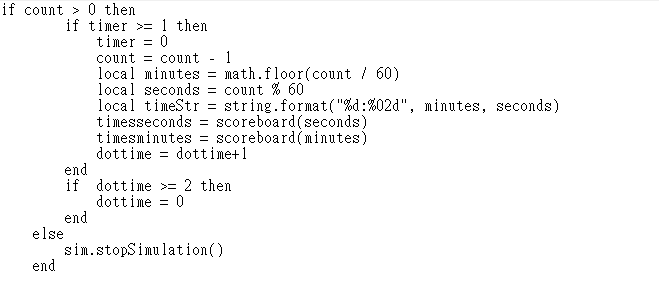
\includegraphics[width=12cm]{8}
\caption{\Large 時間到則停止遊戲}\label{時間到則停止遊戲}
\end{center}
\end{figure} 
\
這個函式,如(圖.\ref{時間到則停止遊戲})包含一個條件語句。首先檢查 count 是否大於 0,如果是,則執行以下操作:\\
檢查 timer 是否大於等於 1,如果是,則將 timer 重置為 0,並將 count 減一。\\
根據 count 計算出分鐘數和秒數,並使用 string.format 函式將其格式化為 分鐘:秒 的字符串形式。\\
將秒數和分鐘數分別轉換為十位數和個位數,並將結果分別存儲在 timesseconds 和 timesminutes 中。
將 dottime 加一。\\
接下來,檢查 dottime 是否大於等於 2,如果是,則將 dottime 重置為 0。\\
如果 count 小於等於 0,則執行 sim.stopSimulation函式停止仿真。\\
\section{回復記分板顏色}
\begin{figure}[htbp!]
\begin{center}
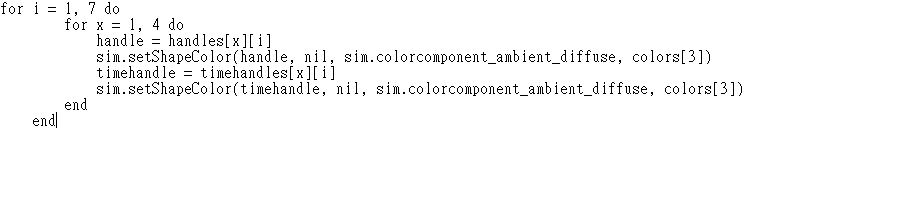
\includegraphics[width=12cm]{9}
\caption{\Large 回復記分板顏色}\label{回復記分板顏色}
\end{center}
\end{figure} 
\
這個函式,如(圖.\ref{回復記分板顏色})使用兩個嵌套的迴圈。外層迴圈遍歷 i 從 1 到 7 的值,內層迴圈遍歷 x 從 1 到 4 的值。\\
對於每一個 i 和 x 的組合,執行以下操作:\\
從 handles 中獲取 handle 的值。
使用 sim.setShapeColor 函式將 handle 的形狀顏色設置為 colors3。
從 timehandles 中獲取 timehandle 的值。
使用 sim.setShapeColor 函式將 timehandle 的形狀顏色設置為 colors3。
換句話說,這段代碼將遍歷一個二維數組 handles 和 timehandles,並將相應的形狀顏色設置為 colors3。\\

\end{document}
